% Created by tikzDevice version 0.12.6 on 2026-08-08 12:11:18
% !TEX encoding = UTF-8 Unicode
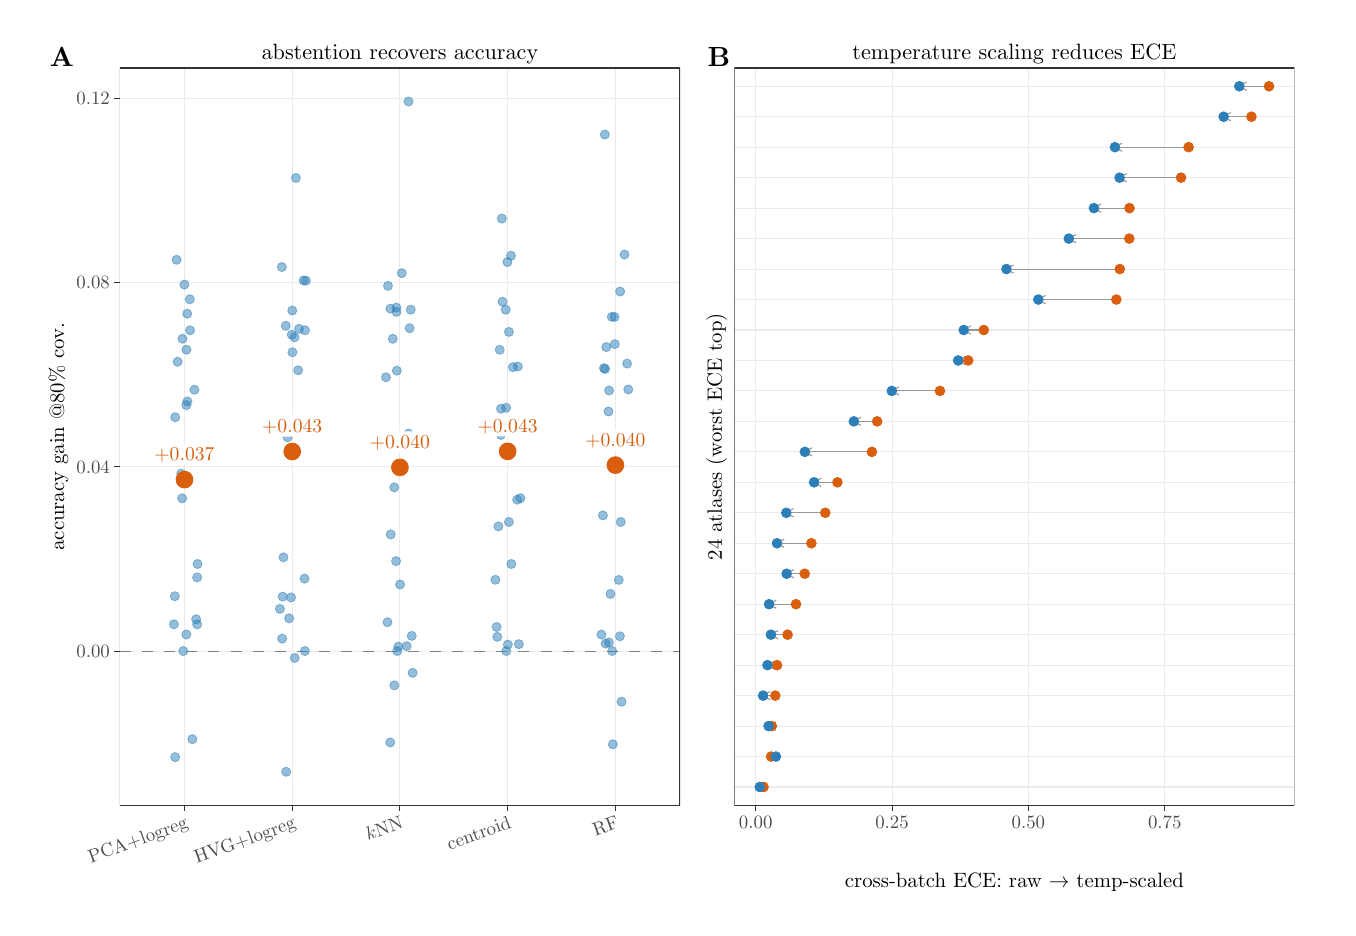
\begin{tikzpicture}[x=1pt,y=1pt]
\definecolor{fillColor}{RGB}{255,255,255}
\path[use as bounding box,fill=fillColor,fill opacity=0.00] (0,0) rectangle (469.75,317.99);
\begin{scope}
\path[clip] (  0.00,  0.00) rectangle (469.75,317.99);
\definecolor{drawColor}{RGB}{255,255,255}
\definecolor{fillColor}{RGB}{255,255,255}

\path[draw=drawColor,line width= 0.4pt,line join=round,line cap=round,fill=fillColor] ( -0.00,  0.00) rectangle (469.76,317.99);
\end{scope}
\begin{scope}
\path[clip] (  4.00,  3.00) rectangle (241.72,314.99);
\definecolor{drawColor}{RGB}{255,255,255}
\definecolor{fillColor}{RGB}{255,255,255}

\path[draw=drawColor,line width= 0.4pt,line join=round,line cap=round,fill=fillColor] (  4.00,  3.00) rectangle (241.72,314.99);
\end{scope}
\begin{scope}
\path[clip] (241.72,  3.00) rectangle (463.76,314.99);
\definecolor{drawColor}{RGB}{255,255,255}
\definecolor{fillColor}{RGB}{255,255,255}

\path[draw=drawColor,line width= 0.4pt,line join=round,line cap=round,fill=fillColor] (241.72,  3.00) rectangle (463.75,314.99);
\end{scope}
\begin{scope}
\path[clip] ( 33.31, 37.00) rectangle (235.72,303.42);
\definecolor{fillColor}{RGB}{255,255,255}

\path[fill=fillColor] ( 33.31, 37.00) rectangle (235.72,303.42);
\definecolor{drawColor}{gray}{0.92}

\path[draw=drawColor,line width= 0.4pt,line join=round] ( 33.31, 92.73) --
	(235.72, 92.73);

\path[draw=drawColor,line width= 0.4pt,line join=round] ( 33.31,159.34) --
	(235.72,159.34);

\path[draw=drawColor,line width= 0.4pt,line join=round] ( 33.31,225.94) --
	(235.72,225.94);

\path[draw=drawColor,line width= 0.4pt,line join=round] ( 33.31,292.54) --
	(235.72,292.54);

\path[draw=drawColor,line width= 0.4pt,line join=round] ( 56.66, 37.00) --
	( 56.66,303.42);

\path[draw=drawColor,line width= 0.4pt,line join=round] ( 95.59, 37.00) --
	( 95.59,303.42);

\path[draw=drawColor,line width= 0.4pt,line join=round] (134.51, 37.00) --
	(134.51,303.42);

\path[draw=drawColor,line width= 0.4pt,line join=round] (173.44, 37.00) --
	(173.44,303.42);

\path[draw=drawColor,line width= 0.4pt,line join=round] (212.37, 37.00) --
	(212.37,303.42);
\definecolor{drawColor}{gray}{0.50}

\path[draw=drawColor,line width= 0.4pt,dash pattern=on 4pt off 4pt ,line join=round] ( 33.31, 92.73) -- (235.72, 92.73);
\definecolor{drawColor}{RGB}{44,127,184}
\definecolor{fillColor}{RGB}{44,127,184}

\path[draw=drawColor,draw opacity=0.50,line width= 0.3pt,line join=round,line cap=round,fill=fillColor,fill opacity=0.50] ( 53.30, 54.40) circle (  1.65);

\path[draw=drawColor,draw opacity=0.50,line width= 0.3pt,line join=round,line cap=round,fill=fillColor,fill opacity=0.50] ( 96.49, 90.24) circle (  1.65);

\path[draw=drawColor,draw opacity=0.50,line width= 0.3pt,line join=round,line cap=round,fill=fillColor,fill opacity=0.50] (136.95, 94.49) circle (  1.65);

\path[draw=drawColor,draw opacity=0.50,line width= 0.3pt,line join=round,line cap=round,fill=fillColor,fill opacity=0.50] (169.70, 97.87) circle (  1.65);

\path[draw=drawColor,draw opacity=0.50,line width= 0.3pt,line join=round,line cap=round,fill=fillColor,fill opacity=0.50] (213.99, 98.07) circle (  1.65);

\path[draw=drawColor,draw opacity=0.50,line width= 0.3pt,line join=round,line cap=round,fill=fillColor,fill opacity=0.50] ( 61.23,119.34) circle (  1.65);

\path[draw=drawColor,draw opacity=0.50,line width= 0.3pt,line join=round,line cap=round,fill=fillColor,fill opacity=0.50] (100.05,118.91) circle (  1.65);

\path[draw=drawColor,draw opacity=0.50,line width= 0.3pt,line join=round,line cap=round,fill=fillColor,fill opacity=0.50] (134.55,116.77) circle (  1.65);

\path[draw=drawColor,draw opacity=0.50,line width= 0.3pt,line join=round,line cap=round,fill=fillColor,fill opacity=0.50] (169.01,118.48) circle (  1.65);

\path[draw=drawColor,draw opacity=0.50,line width= 0.3pt,line join=round,line cap=round,fill=fillColor,fill opacity=0.50] (210.59,113.37) circle (  1.65);

\path[draw=drawColor,draw opacity=0.50,line width= 0.3pt,line join=round,line cap=round,fill=fillColor,fill opacity=0.50] ( 55.83,147.92) circle (  1.65);

\path[draw=drawColor,draw opacity=0.50,line width= 0.3pt,line join=round,line cap=round,fill=fillColor,fill opacity=0.50] ( 92.43,126.59) circle (  1.65);

\path[draw=drawColor,draw opacity=0.50,line width= 0.3pt,line join=round,line cap=round,fill=fillColor,fill opacity=0.50] (137.59,171.30) circle (  1.65);

\path[draw=drawColor,draw opacity=0.50,line width= 0.3pt,line join=round,line cap=round,fill=fillColor,fill opacity=0.50] (173.36,233.30) circle (  1.65);

\path[draw=drawColor,draw opacity=0.50,line width= 0.3pt,line join=round,line cap=round,fill=fillColor,fill opacity=0.50] (207.87,141.74) circle (  1.65);

\path[draw=drawColor,draw opacity=0.50,line width= 0.3pt,line join=round,line cap=round,fill=fillColor,fill opacity=0.50] ( 61.38,124.19) circle (  1.65);

\path[draw=drawColor,draw opacity=0.50,line width= 0.3pt,line join=round,line cap=round,fill=fillColor,fill opacity=0.50] ( 92.15,112.40) circle (  1.65);

\path[draw=drawColor,draw opacity=0.50,line width= 0.3pt,line join=round,line cap=round,fill=fillColor,fill opacity=0.50] (131.18,134.87) circle (  1.65);

\path[draw=drawColor,draw opacity=0.50,line width= 0.3pt,line join=round,line cap=round,fill=fillColor,fill opacity=0.50] (173.89,139.37) circle (  1.65);

\path[draw=drawColor,draw opacity=0.50,line width= 0.3pt,line join=round,line cap=round,fill=fillColor,fill opacity=0.50] (214.32,139.38) circle (  1.65);

\path[draw=drawColor,draw opacity=0.50,line width= 0.3pt,line join=round,line cap=round,fill=fillColor,fill opacity=0.50] ( 55.48,156.84) circle (  1.65);

\path[draw=drawColor,draw opacity=0.50,line width= 0.3pt,line join=round,line cap=round,fill=fillColor,fill opacity=0.50] ( 98.03,174.21) circle (  1.65);

\path[draw=drawColor,draw opacity=0.50,line width= 0.3pt,line join=round,line cap=round,fill=fillColor,fill opacity=0.50] (138.02,209.38) circle (  1.65);

\path[draw=drawColor,draw opacity=0.50,line width= 0.3pt,line join=round,line cap=round,fill=fillColor,fill opacity=0.50] (171.35,249.00) circle (  1.65);

\path[draw=drawColor,draw opacity=0.50,line width= 0.3pt,line join=round,line cap=round,fill=fillColor,fill opacity=0.50] (209.07,202.56) circle (  1.65);

\path[draw=drawColor,draw opacity=0.50,line width= 0.3pt,line join=round,line cap=round,fill=fillColor,fill opacity=0.50] ( 57.33, 98.71) circle (  1.65);

\path[draw=drawColor,draw opacity=0.50,line width= 0.3pt,line join=round,line cap=round,fill=fillColor,fill opacity=0.50] ( 91.95, 97.22) circle (  1.65);

\path[draw=drawColor,draw opacity=0.50,line width= 0.3pt,line join=round,line cap=round,fill=fillColor,fill opacity=0.50] (138.79, 98.21) circle (  1.65);

\path[draw=drawColor,draw opacity=0.50,line width= 0.3pt,line join=round,line cap=round,fill=fillColor,fill opacity=0.50] (177.50, 95.23) circle (  1.65);

\path[draw=drawColor,draw opacity=0.50,line width= 0.3pt,line join=round,line cap=round,fill=fillColor,fill opacity=0.50] (210.04, 95.83) circle (  1.65);

\path[draw=drawColor,draw opacity=0.50,line width= 0.3pt,line join=round,line cap=round,fill=fillColor,fill opacity=0.50] ( 58.60,219.85) circle (  1.65);

\path[draw=drawColor,draw opacity=0.50,line width= 0.3pt,line join=round,line cap=round,fill=fillColor,fill opacity=0.50] ( 95.60,215.77) circle (  1.65);

\path[draw=drawColor,draw opacity=0.50,line width= 0.3pt,line join=round,line cap=round,fill=fillColor,fill opacity=0.50] (129.47,191.66) circle (  1.65);

\path[draw=drawColor,draw opacity=0.50,line width= 0.3pt,line join=round,line cap=round,fill=fillColor,fill opacity=0.50] (174.63,235.59) circle (  1.65);

\path[draw=drawColor,draw opacity=0.50,line width= 0.3pt,line join=round,line cap=round,fill=fillColor,fill opacity=0.50] (214.09,222.65) circle (  1.65);

\path[draw=drawColor,draw opacity=0.50,line width= 0.3pt,line join=round,line cap=round,fill=fillColor,fill opacity=0.50] ( 60.88,104.21) circle (  1.65);

\path[draw=drawColor,draw opacity=0.50,line width= 0.3pt,line join=round,line cap=round,fill=fillColor,fill opacity=0.50] ( 94.48,104.56) circle (  1.65);

\path[draw=drawColor,draw opacity=0.50,line width= 0.3pt,line join=round,line cap=round,fill=fillColor,fill opacity=0.50] (130.01,103.16) circle (  1.65);

\path[draw=drawColor,draw opacity=0.50,line width= 0.3pt,line join=round,line cap=round,fill=fillColor,fill opacity=0.50] (169.44,101.42) circle (  1.65);

\path[draw=drawColor,draw opacity=0.50,line width= 0.3pt,line join=round,line cap=round,fill=fillColor,fill opacity=0.50] (207.32, 98.69) circle (  1.65);

\path[draw=drawColor,draw opacity=0.50,line width= 0.3pt,line join=round,line cap=round,fill=fillColor,fill opacity=0.50] ( 54.18,197.25) circle (  1.65);

\path[draw=drawColor,draw opacity=0.50,line width= 0.3pt,line join=round,line cap=round,fill=fillColor,fill opacity=0.50] (100.54,226.55) circle (  1.65);

\path[draw=drawColor,draw opacity=0.50,line width= 0.3pt,line join=round,line cap=round,fill=fillColor,fill opacity=0.50] (132.46,151.89) circle (  1.65);

\path[draw=drawColor,draw opacity=0.50,line width= 0.3pt,line join=round,line cap=round,fill=fillColor,fill opacity=0.50] (176.88,147.43) circle (  1.65);

\path[draw=drawColor,draw opacity=0.50,line width= 0.3pt,line join=round,line cap=round,fill=fillColor,fill opacity=0.50] (210.09,186.88) circle (  1.65);

\path[draw=drawColor,draw opacity=0.50,line width= 0.3pt,line join=round,line cap=round,fill=fillColor,fill opacity=0.50] ( 57.33,181.61) circle (  1.65);

\path[draw=drawColor,draw opacity=0.50,line width= 0.3pt,line join=round,line cap=round,fill=fillColor,fill opacity=0.50] ( 93.26,210.25) circle (  1.65);

\path[draw=drawColor,draw opacity=0.50,line width= 0.3pt,line join=round,line cap=round,fill=fillColor,fill opacity=0.50] (131.92,205.56) circle (  1.65);

\path[draw=drawColor,draw opacity=0.50,line width= 0.3pt,line join=round,line cap=round,fill=fillColor,fill opacity=0.50] (171.02,180.29) circle (  1.65);

\path[draw=drawColor,draw opacity=0.50,line width= 0.3pt,line join=round,line cap=round,fill=fillColor,fill opacity=0.50] (212.16,203.64) circle (  1.65);

\path[draw=drawColor,draw opacity=0.50,line width= 0.3pt,line join=round,line cap=round,fill=fillColor,fill opacity=0.50] ( 57.65,214.63) circle (  1.65);

\path[draw=drawColor,draw opacity=0.50,line width= 0.3pt,line join=round,line cap=round,fill=fillColor,fill opacity=0.50] ( 99.70,226.65) circle (  1.65);

\path[draw=drawColor,draw opacity=0.50,line width= 0.3pt,line join=round,line cap=round,fill=fillColor,fill opacity=0.50] (135.17,229.27) circle (  1.65);

\path[draw=drawColor,draw opacity=0.50,line width= 0.3pt,line join=round,line cap=round,fill=fillColor,fill opacity=0.50] (177.12,195.54) circle (  1.65);

\path[draw=drawColor,draw opacity=0.50,line width= 0.3pt,line join=round,line cap=round,fill=fillColor,fill opacity=0.50] (215.67,236.00) circle (  1.65);

\path[draw=drawColor,draw opacity=0.50,line width= 0.3pt,line join=round,line cap=round,fill=fillColor,fill opacity=0.50] ( 56.64,225.14) circle (  1.65);

\path[draw=drawColor,draw opacity=0.50,line width= 0.3pt,line join=round,line cap=round,fill=fillColor,fill opacity=0.50] ( 95.66,200.70) circle (  1.65);

\path[draw=drawColor,draw opacity=0.50,line width= 0.3pt,line join=round,line cap=round,fill=fillColor,fill opacity=0.50] (131.08,216.46) circle (  1.65);

\path[draw=drawColor,draw opacity=0.50,line width= 0.3pt,line join=round,line cap=round,fill=fillColor,fill opacity=0.50] (176.77,174.80) circle (  1.65);

\path[draw=drawColor,draw opacity=0.50,line width= 0.3pt,line join=round,line cap=round,fill=fillColor,fill opacity=0.50] (208.65,194.66) circle (  1.65);

\path[draw=drawColor,draw opacity=0.50,line width= 0.3pt,line join=round,line cap=round,fill=fillColor,fill opacity=0.50] ( 56.22, 92.73) circle (  1.65);

\path[draw=drawColor,draw opacity=0.50,line width= 0.3pt,line join=round,line cap=round,fill=fillColor,fill opacity=0.50] (100.17, 92.73) circle (  1.65);

\path[draw=drawColor,draw opacity=0.50,line width= 0.3pt,line join=round,line cap=round,fill=fillColor,fill opacity=0.50] (133.53, 92.73) circle (  1.65);

\path[draw=drawColor,draw opacity=0.50,line width= 0.3pt,line join=round,line cap=round,fill=fillColor,fill opacity=0.50] (172.93, 92.73) circle (  1.65);

\path[draw=drawColor,draw opacity=0.50,line width= 0.3pt,line join=round,line cap=round,fill=fillColor,fill opacity=0.50] (211.22, 92.73) circle (  1.65);

\path[draw=drawColor,draw opacity=0.50,line width= 0.3pt,line join=round,line cap=round,fill=fillColor,fill opacity=0.50] ( 52.85,102.40) circle (  1.65);

\path[draw=drawColor,draw opacity=0.50,line width= 0.3pt,line join=round,line cap=round,fill=fillColor,fill opacity=0.50] ( 93.93,169.95) circle (  1.65);

\path[draw=drawColor,draw opacity=0.50,line width= 0.3pt,line join=round,line cap=round,fill=fillColor,fill opacity=0.50] (131.03, 59.70) circle (  1.65);

\path[draw=drawColor,draw opacity=0.50,line width= 0.3pt,line join=round,line cap=round,fill=fillColor,fill opacity=0.50] (178.07,147.98) circle (  1.65);

\path[draw=drawColor,draw opacity=0.50,line width= 0.3pt,line join=round,line cap=round,fill=fillColor,fill opacity=0.50] (213.60,118.44) circle (  1.65);

\path[draw=drawColor,draw opacity=0.50,line width= 0.3pt,line join=round,line cap=round,fill=fillColor,fill opacity=0.50] ( 58.67,208.64) circle (  1.65);

\path[draw=drawColor,draw opacity=0.50,line width= 0.3pt,line join=round,line cap=round,fill=fillColor,fill opacity=0.50] ( 95.43,207.05) circle (  1.65);

\path[draw=drawColor,draw opacity=0.50,line width= 0.3pt,line join=round,line cap=round,fill=fillColor,fill opacity=0.50] (133.29,215.28) circle (  1.65);

\path[draw=drawColor,draw opacity=0.50,line width= 0.3pt,line join=round,line cap=round,fill=fillColor,fill opacity=0.50] (171.59,218.95) circle (  1.65);

\path[draw=drawColor,draw opacity=0.50,line width= 0.3pt,line join=round,line cap=round,fill=fillColor,fill opacity=0.50] (208.23,194.96) circle (  1.65);

\path[draw=drawColor,draw opacity=0.50,line width= 0.3pt,line join=round,line cap=round,fill=fillColor,fill opacity=0.50] ( 53.30,177.22) circle (  1.65);

\path[draw=drawColor,draw opacity=0.50,line width= 0.3pt,line join=round,line cap=round,fill=fillColor,fill opacity=0.50] ( 91.85,231.49) circle (  1.65);

\path[draw=drawColor,draw opacity=0.50,line width= 0.3pt,line join=round,line cap=round,fill=fillColor,fill opacity=0.50] (138.43,216.07) circle (  1.65);

\path[draw=drawColor,draw opacity=0.50,line width= 0.3pt,line join=round,line cap=round,fill=fillColor,fill opacity=0.50] (173.91,208.06) circle (  1.65);

\path[draw=drawColor,draw opacity=0.50,line width= 0.3pt,line join=round,line cap=round,fill=fillColor,fill opacity=0.50] (217.03,187.26) circle (  1.65);

\path[draw=drawColor,draw opacity=0.50,line width= 0.3pt,line join=round,line cap=round,fill=fillColor,fill opacity=0.50] ( 59.50, 60.90) circle (  1.65);

\path[draw=drawColor,draw opacity=0.50,line width= 0.3pt,line join=round,line cap=round,fill=fillColor,fill opacity=0.50] ( 93.40, 49.11) circle (  1.65);

\path[draw=drawColor,draw opacity=0.50,line width= 0.3pt,line join=round,line cap=round,fill=fillColor,fill opacity=0.50] (132.49, 80.34) circle (  1.65);

\path[draw=drawColor,draw opacity=0.50,line width= 0.3pt,line join=round,line cap=round,fill=fillColor,fill opacity=0.50] (173.51, 95.07) circle (  1.65);

\path[draw=drawColor,draw opacity=0.50,line width= 0.3pt,line join=round,line cap=round,fill=fillColor,fill opacity=0.50] (211.45, 59.04) circle (  1.65);

\path[draw=drawColor,draw opacity=0.50,line width= 0.3pt,line join=round,line cap=round,fill=fillColor,fill opacity=0.50] ( 57.73,182.95) circle (  1.65);

\path[draw=drawColor,draw opacity=0.50,line width= 0.3pt,line join=round,line cap=round,fill=fillColor,fill opacity=0.50] ( 98.06,209.16) circle (  1.65);

\path[draw=drawColor,draw opacity=0.50,line width= 0.3pt,line join=round,line cap=round,fill=fillColor,fill opacity=0.50] (133.11,125.24) circle (  1.65);

\path[draw=drawColor,draw opacity=0.50,line width= 0.3pt,line join=round,line cap=round,fill=fillColor,fill opacity=0.50] (172.87,180.63) circle (  1.65);

\path[draw=drawColor,draw opacity=0.50,line width= 0.3pt,line join=round,line cap=round,fill=fillColor,fill opacity=0.50] (209.88,179.30) circle (  1.65);

\path[draw=drawColor,draw opacity=0.50,line width= 0.3pt,line join=round,line cap=round,fill=fillColor,fill opacity=0.50] ( 55.94,205.57) circle (  1.65);

\path[draw=drawColor,draw opacity=0.50,line width= 0.3pt,line join=round,line cap=round,fill=fillColor,fill opacity=0.50] (100.20,208.64) circle (  1.65);

\path[draw=drawColor,draw opacity=0.50,line width= 0.3pt,line join=round,line cap=round,fill=fillColor,fill opacity=0.50] (130.18,224.70) circle (  1.65);

\path[draw=drawColor,draw opacity=0.50,line width= 0.3pt,line join=round,line cap=round,fill=fillColor,fill opacity=0.50] (172.73,216.05) circle (  1.65);

\path[draw=drawColor,draw opacity=0.50,line width= 0.3pt,line join=round,line cap=round,fill=fillColor,fill opacity=0.50] (216.61,196.61) circle (  1.65);

\path[draw=drawColor,draw opacity=0.50,line width= 0.3pt,line join=round,line cap=round,fill=fillColor,fill opacity=0.50] ( 61.24,102.39) circle (  1.65);

\path[draw=drawColor,draw opacity=0.50,line width= 0.3pt,line join=round,line cap=round,fill=fillColor,fill opacity=0.50] ( 91.14,107.97) circle (  1.65);

\path[draw=drawColor,draw opacity=0.50,line width= 0.3pt,line join=round,line cap=round,fill=fillColor,fill opacity=0.50] (139.10, 84.84) circle (  1.65);

\path[draw=drawColor,draw opacity=0.50,line width= 0.3pt,line join=round,line cap=round,fill=fillColor,fill opacity=0.50] (170.08,137.76) circle (  1.65);

\path[draw=drawColor,draw opacity=0.50,line width= 0.3pt,line join=round,line cap=round,fill=fillColor,fill opacity=0.50] (214.59, 74.42) circle (  1.65);

\path[draw=drawColor,draw opacity=0.50,line width= 0.3pt,line join=round,line cap=round,fill=fillColor,fill opacity=0.50] ( 60.25,187.14) circle (  1.65);

\path[draw=drawColor,draw opacity=0.50,line width= 0.3pt,line join=round,line cap=round,fill=fillColor,fill opacity=0.50] ( 97.72,194.19) circle (  1.65);

\path[draw=drawColor,draw opacity=0.50,line width= 0.3pt,line join=round,line cap=round,fill=fillColor,fill opacity=0.50] (133.23,216.83) circle (  1.65);

\path[draw=drawColor,draw opacity=0.50,line width= 0.3pt,line join=round,line cap=round,fill=fillColor,fill opacity=0.50] (170.57,201.59) circle (  1.65);

\path[draw=drawColor,draw opacity=0.50,line width= 0.3pt,line join=round,line cap=round,fill=fillColor,fill opacity=0.50] (211.08,213.49) circle (  1.65);

\path[draw=drawColor,draw opacity=0.50,line width= 0.3pt,line join=round,line cap=round,fill=fillColor,fill opacity=0.50] ( 57.37,201.62) circle (  1.65);

\path[draw=drawColor,draw opacity=0.50,line width= 0.3pt,line join=round,line cap=round,fill=fillColor,fill opacity=0.50] ( 96.43,206.10) circle (  1.65);

\path[draw=drawColor,draw opacity=0.50,line width= 0.3pt,line join=round,line cap=round,fill=fillColor,fill opacity=0.50] (133.39,194.04) circle (  1.65);

\path[draw=drawColor,draw opacity=0.50,line width= 0.3pt,line join=round,line cap=round,fill=fillColor,fill opacity=0.50] (171.02,170.81) circle (  1.65);

\path[draw=drawColor,draw opacity=0.50,line width= 0.3pt,line join=round,line cap=round,fill=fillColor,fill opacity=0.50] (212.06,213.47) circle (  1.65);

\path[draw=drawColor,draw opacity=0.50,line width= 0.3pt,line join=round,line cap=round,fill=fillColor,fill opacity=0.50] ( 53.80,234.11) circle (  1.65);

\path[draw=drawColor,draw opacity=0.50,line width= 0.3pt,line join=round,line cap=round,fill=fillColor,fill opacity=0.50] ( 96.92,263.69) circle (  1.65);

\path[draw=drawColor,draw opacity=0.50,line width= 0.3pt,line join=round,line cap=round,fill=fillColor,fill opacity=0.50] (137.62,291.31) circle (  1.65);

\path[draw=drawColor,draw opacity=0.50,line width= 0.3pt,line join=round,line cap=round,fill=fillColor,fill opacity=0.50] (175.35,195.31) circle (  1.65);

\path[draw=drawColor,draw opacity=0.50,line width= 0.3pt,line join=round,line cap=round,fill=fillColor,fill opacity=0.50] (208.56,279.36) circle (  1.65);

\path[draw=drawColor,draw opacity=0.50,line width= 0.3pt,line join=round,line cap=round,fill=fillColor,fill opacity=0.50] ( 53.18,112.55) circle (  1.65);

\path[draw=drawColor,draw opacity=0.50,line width= 0.3pt,line join=round,line cap=round,fill=fillColor,fill opacity=0.50] ( 95.19,112.10) circle (  1.65);

\path[draw=drawColor,draw opacity=0.50,line width= 0.3pt,line join=round,line cap=round,fill=fillColor,fill opacity=0.50] (133.95, 94.34) circle (  1.65);

\path[draw=drawColor,draw opacity=0.50,line width= 0.3pt,line join=round,line cap=round,fill=fillColor,fill opacity=0.50] (174.78,124.19) circle (  1.65);

\path[draw=drawColor,draw opacity=0.50,line width= 0.3pt,line join=round,line cap=round,fill=fillColor,fill opacity=0.50] (208.84, 95.44) circle (  1.65);
\definecolor{drawColor}{RGB}{217,95,14}
\definecolor{fillColor}{RGB}{217,95,14}

\path[draw=drawColor,line width= 0.3pt,line join=round,line cap=round,fill=fillColor] ( 56.66,154.68) circle (  3.04);

\path[draw=drawColor,line width= 0.3pt,line join=round,line cap=round,fill=fillColor] ( 95.59,164.84) circle (  3.04);

\path[draw=drawColor,line width= 0.3pt,line join=round,line cap=round,fill=fillColor] (134.51,159.10) circle (  3.04);

\path[draw=drawColor,line width= 0.3pt,line join=round,line cap=round,fill=fillColor] (173.44,164.89) circle (  3.04);

\path[draw=drawColor,line width= 0.3pt,line join=round,line cap=round,fill=fillColor] (212.37,159.92) circle (  3.04);
\definecolor{fillColor}{RGB}{255,255,255}

\path[fill=fillColor] ( 46.49,160.05) --
	( 66.84,160.05) --
	( 66.79,160.05) --
	( 67.00,160.06) --
	( 67.20,160.10) --
	( 67.39,160.17) --
	( 67.57,160.27) --
	( 67.73,160.40) --
	( 67.87,160.56) --
	( 67.98,160.73) --
	( 68.06,160.92) --
	( 68.11,161.13) --
	( 68.13,161.33) --
	( 68.13,161.33) --
	( 68.13,166.43) --
	( 68.13,166.43) --
	( 68.11,166.63) --
	( 68.06,166.83) --
	( 67.98,167.02) --
	( 67.87,167.20) --
	( 67.73,167.35) --
	( 67.57,167.48) --
	( 67.39,167.59) --
	( 67.20,167.66) --
	( 67.00,167.70) --
	( 66.84,167.71) --
	( 46.49,167.71) --
	( 46.64,167.70) --
	( 46.43,167.71) --
	( 46.23,167.68) --
	( 46.03,167.63) --
	( 45.84,167.54) --
	( 45.67,167.42) --
	( 45.52,167.28) --
	( 45.40,167.11) --
	( 45.30,166.93) --
	( 45.24,166.73) --
	( 45.20,166.53) --
	( 45.20,166.43) --
	( 45.20,161.33) --
	( 45.20,161.43) --
	( 45.20,161.23) --
	( 45.24,161.02) --
	( 45.30,160.83) --
	( 45.40,160.64) --
	( 45.52,160.48) --
	( 45.67,160.34) --
	( 45.84,160.22) --
	( 46.03,160.13) --
	( 46.23,160.07) --
	( 46.43,160.05) --
	cycle;
\end{scope}
\begin{scope}
\path[clip] ( 33.31, 37.00) rectangle (235.72,303.42);
\definecolor{drawColor}{RGB}{217,95,14}

\node[text=drawColor,anchor=base,inner sep=0pt, outer sep=0pt, scale=  0.71] at ( 56.66,161.43) {+0.037};
\end{scope}
\begin{scope}
\path[clip] ( 33.31, 37.00) rectangle (235.72,303.42);
\definecolor{fillColor}{RGB}{255,255,255}

\path[fill=fillColor] ( 85.41,170.21) --
	(105.77,170.21) --
	(105.72,170.21) --
	(105.92,170.22) --
	(106.13,170.26) --
	(106.32,170.33) --
	(106.50,170.44) --
	(106.66,170.57) --
	(106.80,170.72) --
	(106.91,170.90) --
	(106.99,171.09) --
	(107.04,171.29) --
	(107.05,171.49) --
	(107.05,171.49) --
	(107.05,176.59) --
	(107.05,176.59) --
	(107.04,176.79) --
	(106.99,176.99) --
	(106.91,177.18) --
	(106.80,177.36) --
	(106.66,177.51) --
	(106.50,177.64) --
	(106.32,177.75) --
	(106.13,177.82) --
	(105.92,177.86) --
	(105.77,177.87) --
	( 85.41,177.87) --
	( 85.57,177.86) --
	( 85.36,177.87) --
	( 85.15,177.85) --
	( 84.95,177.79) --
	( 84.77,177.70) --
	( 84.60,177.58) --
	( 84.45,177.44) --
	( 84.32,177.27) --
	( 84.23,177.09) --
	( 84.16,176.89) --
	( 84.13,176.69) --
	( 84.13,176.59) --
	( 84.13,171.49) --
	( 84.13,171.60) --
	( 84.13,171.39) --
	( 84.16,171.19) --
	( 84.23,170.99) --
	( 84.32,170.81) --
	( 84.45,170.64) --
	( 84.60,170.50) --
	( 84.77,170.38) --
	( 84.95,170.29) --
	( 85.15,170.23) --
	( 85.36,170.21) --
	cycle;
\end{scope}
\begin{scope}
\path[clip] ( 33.31, 37.00) rectangle (235.72,303.42);
\definecolor{drawColor}{RGB}{217,95,14}

\node[text=drawColor,anchor=base,inner sep=0pt, outer sep=0pt, scale=  0.71] at ( 95.59,171.59) {+0.043};
\end{scope}
\begin{scope}
\path[clip] ( 33.31, 37.00) rectangle (235.72,303.42);
\definecolor{fillColor}{RGB}{255,255,255}

\path[fill=fillColor] (124.34,164.47) --
	(144.69,164.47) --
	(144.64,164.47) --
	(144.85,164.48) --
	(145.05,164.52) --
	(145.25,164.59) --
	(145.42,164.69) --
	(145.58,164.83) --
	(145.72,164.98) --
	(145.83,165.15) --
	(145.91,165.35) --
	(145.96,165.55) --
	(145.98,165.75) --
	(145.98,165.75) --
	(145.98,170.85) --
	(145.98,170.85) --
	(145.96,171.05) --
	(145.91,171.25) --
	(145.83,171.44) --
	(145.72,171.62) --
	(145.58,171.77) --
	(145.42,171.90) --
	(145.25,172.01) --
	(145.05,172.08) --
	(144.85,172.12) --
	(144.69,172.13) --
	(124.34,172.13) --
	(124.49,172.12) --
	(124.28,172.13) --
	(124.08,172.11) --
	(123.88,172.05) --
	(123.69,171.96) --
	(123.52,171.84) --
	(123.37,171.70) --
	(123.25,171.53) --
	(123.15,171.35) --
	(123.09,171.15) --
	(123.05,170.95) --
	(123.05,170.85) --
	(123.05,165.75) --
	(123.05,165.86) --
	(123.05,165.65) --
	(123.09,165.44) --
	(123.15,165.25) --
	(123.25,165.07) --
	(123.37,164.90) --
	(123.52,164.76) --
	(123.69,164.64) --
	(123.88,164.55) --
	(124.08,164.49) --
	(124.28,164.47) --
	cycle;
\end{scope}
\begin{scope}
\path[clip] ( 33.31, 37.00) rectangle (235.72,303.42);
\definecolor{drawColor}{RGB}{217,95,14}

\node[text=drawColor,anchor=base,inner sep=0pt, outer sep=0pt, scale=  0.71] at (134.51,165.85) {+0.040};
\end{scope}
\begin{scope}
\path[clip] ( 33.31, 37.00) rectangle (235.72,303.42);
\definecolor{fillColor}{RGB}{255,255,255}

\path[fill=fillColor] (163.26,170.26) --
	(183.62,170.26) --
	(183.57,170.26) --
	(183.77,170.27) --
	(183.98,170.31) --
	(184.17,170.38) --
	(184.35,170.49) --
	(184.51,170.62) --
	(184.65,170.77) --
	(184.76,170.95) --
	(184.84,171.14) --
	(184.89,171.34) --
	(184.90,171.54) --
	(184.90,171.54) --
	(184.90,176.64) --
	(184.90,176.64) --
	(184.89,176.84) --
	(184.84,177.05) --
	(184.76,177.24) --
	(184.65,177.41) --
	(184.51,177.57) --
	(184.35,177.70) --
	(184.17,177.80) --
	(183.98,177.87) --
	(183.77,177.91) --
	(183.62,177.92) --
	(163.26,177.92) --
	(163.42,177.91) --
	(163.21,177.92) --
	(163.00,177.90) --
	(162.80,177.84) --
	(162.62,177.75) --
	(162.45,177.63) --
	(162.30,177.49) --
	(162.17,177.33) --
	(162.08,177.14) --
	(162.01,176.95) --
	(161.98,176.74) --
	(161.98,176.64) --
	(161.98,171.54) --
	(161.98,171.65) --
	(161.98,171.44) --
	(162.01,171.24) --
	(162.08,171.04) --
	(162.17,170.86) --
	(162.30,170.69) --
	(162.45,170.55) --
	(162.62,170.43) --
	(162.80,170.34) --
	(163.00,170.29) --
	(163.21,170.26) --
	cycle;
\end{scope}
\begin{scope}
\path[clip] ( 33.31, 37.00) rectangle (235.72,303.42);
\definecolor{drawColor}{RGB}{217,95,14}

\node[text=drawColor,anchor=base,inner sep=0pt, outer sep=0pt, scale=  0.71] at (173.44,171.64) {+0.043};
\end{scope}
\begin{scope}
\path[clip] ( 33.31, 37.00) rectangle (235.72,303.42);
\definecolor{fillColor}{RGB}{255,255,255}

\path[fill=fillColor] (202.19,165.28) --
	(222.54,165.28) --
	(222.49,165.28) --
	(222.70,165.29) --
	(222.90,165.33) --
	(223.10,165.40) --
	(223.27,165.51) --
	(223.43,165.64) --
	(223.57,165.79) --
	(223.68,165.97) --
	(223.76,166.16) --
	(223.81,166.36) --
	(223.83,166.57) --
	(223.83,166.57) --
	(223.83,171.66) --
	(223.83,171.66) --
	(223.81,171.87) --
	(223.76,172.07) --
	(223.68,172.26) --
	(223.57,172.43) --
	(223.43,172.59) --
	(223.27,172.72) --
	(223.10,172.82) --
	(222.90,172.89) --
	(222.70,172.94) --
	(222.54,172.95) --
	(202.19,172.95) --
	(202.34,172.94) --
	(202.13,172.94) --
	(201.93,172.92) --
	(201.73,172.86) --
	(201.54,172.77) --
	(201.37,172.66) --
	(201.22,172.51) --
	(201.10,172.35) --
	(201.00,172.16) --
	(200.94,171.97) --
	(200.90,171.76) --
	(200.90,171.66) --
	(200.90,166.57) --
	(200.90,166.67) --
	(200.90,166.46) --
	(200.94,166.26) --
	(201.00,166.06) --
	(201.10,165.88) --
	(201.22,165.71) --
	(201.37,165.57) --
	(201.54,165.45) --
	(201.73,165.36) --
	(201.93,165.31) --
	(202.13,165.28) --
	cycle;
\end{scope}
\begin{scope}
\path[clip] ( 33.31, 37.00) rectangle (235.72,303.42);
\definecolor{drawColor}{RGB}{217,95,14}

\node[text=drawColor,anchor=base,inner sep=0pt, outer sep=0pt, scale=  0.71] at (212.37,166.66) {+0.040};
\end{scope}
\begin{scope}
\path[clip] ( 33.31, 37.00) rectangle (235.72,303.42);
\definecolor{drawColor}{gray}{0.20}

\path[draw=drawColor,line width= 0.4pt,line join=round,line cap=round] ( 33.31, 37.00) rectangle (235.72,303.42);
\end{scope}
\begin{scope}
\path[clip] (  0.00,  0.00) rectangle (469.75,317.99);
\definecolor{drawColor}{gray}{0.30}

\node[text=drawColor,anchor=base east,inner sep=0pt, outer sep=0pt, scale=  0.68] at ( 29.71, 90.39) {0.00};

\node[text=drawColor,anchor=base east,inner sep=0pt, outer sep=0pt, scale=  0.68] at ( 29.71,157.00) {0.04};

\node[text=drawColor,anchor=base east,inner sep=0pt, outer sep=0pt, scale=  0.68] at ( 29.71,223.60) {0.08};

\node[text=drawColor,anchor=base east,inner sep=0pt, outer sep=0pt, scale=  0.68] at ( 29.71,290.20) {0.12};
\end{scope}
\begin{scope}
\path[clip] (  0.00,  0.00) rectangle (469.75,317.99);
\definecolor{drawColor}{gray}{0.20}

\path[draw=drawColor,line width= 0.4pt,line join=round] ( 31.31, 92.73) --
	( 33.31, 92.73);

\path[draw=drawColor,line width= 0.4pt,line join=round] ( 31.31,159.34) --
	( 33.31,159.34);

\path[draw=drawColor,line width= 0.4pt,line join=round] ( 31.31,225.94) --
	( 33.31,225.94);

\path[draw=drawColor,line width= 0.4pt,line join=round] ( 31.31,292.54) --
	( 33.31,292.54);
\end{scope}
\begin{scope}
\path[clip] (  0.00,  0.00) rectangle (469.75,317.99);
\definecolor{drawColor}{gray}{0.20}

\path[draw=drawColor,line width= 0.4pt,line join=round] ( 56.66, 35.00) --
	( 56.66, 37.00);

\path[draw=drawColor,line width= 0.4pt,line join=round] ( 95.59, 35.00) --
	( 95.59, 37.00);

\path[draw=drawColor,line width= 0.4pt,line join=round] (134.51, 35.00) --
	(134.51, 37.00);

\path[draw=drawColor,line width= 0.4pt,line join=round] (173.44, 35.00) --
	(173.44, 37.00);

\path[draw=drawColor,line width= 0.4pt,line join=round] (212.37, 35.00) --
	(212.37, 37.00);
\end{scope}
\begin{scope}
\path[clip] (  0.00,  0.00) rectangle (469.75,317.99);
\definecolor{drawColor}{gray}{0.30}

\node[text=drawColor,rotate= 20.00,anchor=base east,inner sep=0pt, outer sep=0pt, scale=  0.68] at ( 58.27, 29.00) {PCA+logreg};

\node[text=drawColor,rotate= 20.00,anchor=base east,inner sep=0pt, outer sep=0pt, scale=  0.68] at ( 97.19, 29.00) {HVG+logreg};

\node[text=drawColor,rotate= 20.00,anchor=base east,inner sep=0pt, outer sep=0pt, scale=  0.68] at (136.12, 29.00) {$k$NN};

\node[text=drawColor,rotate= 20.00,anchor=base east,inner sep=0pt, outer sep=0pt, scale=  0.68] at (175.04, 29.00) {centroid};

\node[text=drawColor,rotate= 20.00,anchor=base east,inner sep=0pt, outer sep=0pt, scale=  0.68] at (213.97, 29.00) {RF};
\end{scope}
\begin{scope}
\path[clip] (  0.00,  0.00) rectangle (469.75,317.99);
\definecolor{drawColor}{RGB}{0,0,0}

\node[text=drawColor,rotate= 90.00,anchor=base,inner sep=0pt, outer sep=0pt, scale=  0.75] at ( 13.17,170.21) {accuracy gain @80\% cov.};
\end{scope}
\begin{scope}
\path[clip] (  0.00,  0.00) rectangle (469.75,317.99);
\definecolor{drawColor}{RGB}{0,0,0}

\node[text=drawColor,anchor=base,inner sep=0pt, outer sep=0pt, scale=  0.80] at (134.51,306.48) {abstention recovers accuracy};
\end{scope}
\begin{scope}
\path[clip] (  0.00,  0.00) rectangle (469.75,317.99);
\definecolor{drawColor}{RGB}{0,0,0}

\node[text=drawColor,anchor=base,inner sep=0pt, outer sep=0pt, scale=  1.00] at ( 12.35,304.11) {\bfseries A};
\end{scope}
\begin{scope}
\path[clip] (255.34, 37.00) rectangle (457.75,303.42);
\definecolor{fillColor}{RGB}{255,255,255}

\path[fill=fillColor] (255.34, 37.00) rectangle (457.75,303.42);
\definecolor{drawColor}{gray}{0.92}

\path[draw=drawColor,line width= 0.4pt,line join=round] (255.34, 43.61) --
	(457.75, 43.61);

\path[draw=drawColor,line width= 0.4pt,line join=round] (255.34, 54.61) --
	(457.75, 54.61);

\path[draw=drawColor,line width= 0.4pt,line join=round] (255.34, 65.62) --
	(457.75, 65.62);

\path[draw=drawColor,line width= 0.4pt,line join=round] (255.34, 76.63) --
	(457.75, 76.63);

\path[draw=drawColor,line width= 0.4pt,line join=round] (255.34, 87.64) --
	(457.75, 87.64);

\path[draw=drawColor,line width= 0.4pt,line join=round] (255.34, 98.65) --
	(457.75, 98.65);

\path[draw=drawColor,line width= 0.4pt,line join=round] (255.34,109.66) --
	(457.75,109.66);

\path[draw=drawColor,line width= 0.4pt,line join=round] (255.34,120.67) --
	(457.75,120.67);

\path[draw=drawColor,line width= 0.4pt,line join=round] (255.34,131.68) --
	(457.75,131.68);

\path[draw=drawColor,line width= 0.4pt,line join=round] (255.34,142.69) --
	(457.75,142.69);

\path[draw=drawColor,line width= 0.4pt,line join=round] (255.34,153.70) --
	(457.75,153.70);

\path[draw=drawColor,line width= 0.4pt,line join=round] (255.34,164.71) --
	(457.75,164.71);

\path[draw=drawColor,line width= 0.4pt,line join=round] (255.34,175.72) --
	(457.75,175.72);

\path[draw=drawColor,line width= 0.4pt,line join=round] (255.34,186.73) --
	(457.75,186.73);

\path[draw=drawColor,line width= 0.4pt,line join=round] (255.34,197.73) --
	(457.75,197.73);

\path[draw=drawColor,line width= 0.4pt,line join=round] (255.34,208.74) --
	(457.75,208.74);

\path[draw=drawColor,line width= 0.4pt,line join=round] (255.34,219.75) --
	(457.75,219.75);

\path[draw=drawColor,line width= 0.4pt,line join=round] (255.34,230.76) --
	(457.75,230.76);

\path[draw=drawColor,line width= 0.4pt,line join=round] (255.34,241.77) --
	(457.75,241.77);

\path[draw=drawColor,line width= 0.4pt,line join=round] (255.34,252.78) --
	(457.75,252.78);

\path[draw=drawColor,line width= 0.4pt,line join=round] (255.34,263.79) --
	(457.75,263.79);

\path[draw=drawColor,line width= 0.4pt,line join=round] (255.34,274.80) --
	(457.75,274.80);

\path[draw=drawColor,line width= 0.4pt,line join=round] (255.34,285.81) --
	(457.75,285.81);

\path[draw=drawColor,line width= 0.4pt,line join=round] (255.34,296.82) --
	(457.75,296.82);

\path[draw=drawColor,line width= 0.4pt,line join=round] (263.07, 37.00) --
	(263.07,303.42);

\path[draw=drawColor,line width= 0.4pt,line join=round] (312.34, 37.00) --
	(312.34,303.42);

\path[draw=drawColor,line width= 0.4pt,line join=round] (361.61, 37.00) --
	(361.61,303.42);

\path[draw=drawColor,line width= 0.4pt,line join=round] (410.88, 37.00) --
	(410.88,303.42);
\definecolor{drawColor}{gray}{0.60}

\path[draw=drawColor,line width= 0.4pt,line join=round] (442.19,285.81) -- (432.16,285.81);

\path[draw=drawColor,line width= 0.4pt,line join=round] (434.75,287.31) --
	(432.16,285.81) --
	(434.75,284.31);

\path[draw=drawColor,line width= 0.4pt,line join=round] (398.14,252.78) -- (385.29,252.78);

\path[draw=drawColor,line width= 0.4pt,line join=round] (387.88,254.28) --
	(385.29,252.78) --
	(387.88,251.28);

\path[draw=drawColor,line width= 0.4pt,line join=round] (329.65,186.73) -- (312.24,186.73);

\path[draw=drawColor,line width= 0.4pt,line join=round] (314.84,188.23) --
	(312.24,186.73) --
	(314.84,185.23);

\path[draw=drawColor,line width= 0.4pt,line join=round] (265.89, 43.61) -- (264.54, 43.61);

\path[draw=drawColor,line width= 0.4pt,line join=round] (267.14, 45.11) --
	(264.54, 43.61) --
	(267.14, 42.11);

\path[draw=drawColor,line width= 0.4pt,line join=round] (270.16, 76.63) -- (265.75, 76.63);

\path[draw=drawColor,line width= 0.4pt,line join=round] (268.35, 78.13) --
	(265.75, 76.63) --
	(268.35, 75.13);

\path[draw=drawColor,line width= 0.4pt,line join=round] (419.51,274.80) -- (392.88,274.80);

\path[draw=drawColor,line width= 0.4pt,line join=round] (395.48,276.30) --
	(392.88,274.80) --
	(395.48,273.30);

\path[draw=drawColor,line width= 0.4pt,line join=round] (339.87,197.73) -- (336.24,197.73);

\path[draw=drawColor,line width= 0.4pt,line join=round] (338.84,199.23) --
	(336.24,197.73) --
	(338.84,196.23);

\path[draw=drawColor,line width= 0.4pt,line join=round] (394.63,230.76) -- (353.68,230.76);

\path[draw=drawColor,line width= 0.4pt,line join=round] (356.28,232.26) --
	(353.68,230.76) --
	(356.28,229.26);

\path[draw=drawColor,line width= 0.4pt,line join=round] (270.79, 87.64) -- (267.33, 87.64);

\path[draw=drawColor,line width= 0.4pt,line join=round] (269.93, 89.14) --
	(267.33, 87.64) --
	(269.93, 86.14);

\path[draw=drawColor,line width= 0.4pt,line join=round] (292.61,153.70) -- (284.17,153.70);

\path[draw=drawColor,line width= 0.4pt,line join=round] (286.77,155.20) --
	(284.17,153.70) --
	(286.77,152.20);

\path[draw=drawColor,line width= 0.4pt,line join=round] (283.19,131.68) -- (270.77,131.68);

\path[draw=drawColor,line width= 0.4pt,line join=round] (273.36,133.18) --
	(270.77,131.68) --
	(273.36,130.18);

\path[draw=drawColor,line width= 0.4pt,line join=round] (306.97,175.72) -- (298.54,175.72);

\path[draw=drawColor,line width= 0.4pt,line join=round] (301.14,177.22) --
	(298.54,175.72) --
	(301.14,174.22);

\path[draw=drawColor,line width= 0.4pt,line join=round] (448.55,296.82) -- (437.83,296.82);

\path[draw=drawColor,line width= 0.4pt,line join=round] (440.43,298.32) --
	(437.83,296.82) --
	(440.43,295.32);

\path[draw=drawColor,line width= 0.4pt,line join=round] (345.48,208.74) -- (338.24,208.74);

\path[draw=drawColor,line width= 0.4pt,line join=round] (340.84,210.24) --
	(338.24,208.74) --
	(340.84,207.24);

\path[draw=drawColor,line width= 0.4pt,line join=round] (268.67, 54.61) -- (270.37, 54.61);

\path[draw=drawColor,line width= 0.4pt,line join=round] (267.77, 53.11) --
	(270.37, 54.61) --
	(267.77, 56.11);

\path[draw=drawColor,line width= 0.4pt,line join=round] (268.88, 65.62) -- (267.72, 65.62);

\path[draw=drawColor,line width= 0.4pt,line join=round] (270.31, 67.12) --
	(267.72, 65.62) --
	(270.31, 64.12);

\path[draw=drawColor,line width= 0.4pt,line join=round] (416.77,263.79) -- (394.56,263.79);

\path[draw=drawColor,line width= 0.4pt,line join=round] (397.16,265.29) --
	(394.56,263.79) --
	(397.16,262.29);

\path[draw=drawColor,line width= 0.4pt,line join=round] (280.77,120.67) -- (274.26,120.67);

\path[draw=drawColor,line width= 0.4pt,line join=round] (276.86,122.17) --
	(274.26,120.67) --
	(276.86,119.17);

\path[draw=drawColor,line width= 0.4pt,line join=round] (277.64,109.66) -- (267.90,109.66);

\path[draw=drawColor,line width= 0.4pt,line join=round] (270.49,111.16) --
	(267.90,109.66) --
	(270.49,108.16);

\path[draw=drawColor,line width= 0.4pt,line join=round] (393.39,219.75) -- (365.20,219.75);

\path[draw=drawColor,line width= 0.4pt,line join=round] (367.80,221.25) --
	(365.20,219.75) --
	(367.80,218.25);

\path[draw=drawColor,line width= 0.4pt,line join=round] (288.21,142.69) -- (274.13,142.69);

\path[draw=drawColor,line width= 0.4pt,line join=round] (276.73,144.19) --
	(274.13,142.69) --
	(276.73,141.19);

\path[draw=drawColor,line width= 0.4pt,line join=round] (305.06,164.71) -- (280.84,164.71);

\path[draw=drawColor,line width= 0.4pt,line join=round] (283.44,166.21) --
	(280.84,164.71) --
	(283.44,163.21);

\path[draw=drawColor,line width= 0.4pt,line join=round] (274.59, 98.65) -- (268.56, 98.65);

\path[draw=drawColor,line width= 0.4pt,line join=round] (271.16,100.15) --
	(268.56, 98.65) --
	(271.16, 97.15);

\path[draw=drawColor,line width= 0.4pt,line join=round] (398.07,241.77) -- (376.21,241.77);

\path[draw=drawColor,line width= 0.4pt,line join=round] (378.81,243.27) --
	(376.21,241.77) --
	(378.81,240.27);
\definecolor{drawColor}{RGB}{217,95,14}
\definecolor{fillColor}{RGB}{217,95,14}

\path[draw=drawColor,line width= 0.3pt,line join=round,line cap=round,fill=fillColor] (442.19,285.81) circle (  1.76);

\path[draw=drawColor,line width= 0.3pt,line join=round,line cap=round,fill=fillColor] (398.14,252.78) circle (  1.76);

\path[draw=drawColor,line width= 0.3pt,line join=round,line cap=round,fill=fillColor] (329.65,186.73) circle (  1.76);

\path[draw=drawColor,line width= 0.3pt,line join=round,line cap=round,fill=fillColor] (265.89, 43.61) circle (  1.76);

\path[draw=drawColor,line width= 0.3pt,line join=round,line cap=round,fill=fillColor] (270.16, 76.63) circle (  1.76);

\path[draw=drawColor,line width= 0.3pt,line join=round,line cap=round,fill=fillColor] (419.51,274.80) circle (  1.76);

\path[draw=drawColor,line width= 0.3pt,line join=round,line cap=round,fill=fillColor] (339.87,197.73) circle (  1.76);

\path[draw=drawColor,line width= 0.3pt,line join=round,line cap=round,fill=fillColor] (394.63,230.76) circle (  1.76);

\path[draw=drawColor,line width= 0.3pt,line join=round,line cap=round,fill=fillColor] (270.79, 87.64) circle (  1.76);

\path[draw=drawColor,line width= 0.3pt,line join=round,line cap=round,fill=fillColor] (292.61,153.70) circle (  1.76);

\path[draw=drawColor,line width= 0.3pt,line join=round,line cap=round,fill=fillColor] (283.19,131.68) circle (  1.76);

\path[draw=drawColor,line width= 0.3pt,line join=round,line cap=round,fill=fillColor] (306.97,175.72) circle (  1.76);

\path[draw=drawColor,line width= 0.3pt,line join=round,line cap=round,fill=fillColor] (448.55,296.82) circle (  1.76);

\path[draw=drawColor,line width= 0.3pt,line join=round,line cap=round,fill=fillColor] (345.48,208.74) circle (  1.76);

\path[draw=drawColor,line width= 0.3pt,line join=round,line cap=round,fill=fillColor] (268.67, 54.61) circle (  1.76);

\path[draw=drawColor,line width= 0.3pt,line join=round,line cap=round,fill=fillColor] (268.88, 65.62) circle (  1.76);

\path[draw=drawColor,line width= 0.3pt,line join=round,line cap=round,fill=fillColor] (416.77,263.79) circle (  1.76);

\path[draw=drawColor,line width= 0.3pt,line join=round,line cap=round,fill=fillColor] (280.77,120.67) circle (  1.76);

\path[draw=drawColor,line width= 0.3pt,line join=round,line cap=round,fill=fillColor] (277.64,109.66) circle (  1.76);

\path[draw=drawColor,line width= 0.3pt,line join=round,line cap=round,fill=fillColor] (393.39,219.75) circle (  1.76);

\path[draw=drawColor,line width= 0.3pt,line join=round,line cap=round,fill=fillColor] (288.21,142.69) circle (  1.76);

\path[draw=drawColor,line width= 0.3pt,line join=round,line cap=round,fill=fillColor] (305.06,164.71) circle (  1.76);

\path[draw=drawColor,line width= 0.3pt,line join=round,line cap=round,fill=fillColor] (274.59, 98.65) circle (  1.76);

\path[draw=drawColor,line width= 0.3pt,line join=round,line cap=round,fill=fillColor] (398.07,241.77) circle (  1.76);
\definecolor{drawColor}{RGB}{44,127,184}
\definecolor{fillColor}{RGB}{44,127,184}

\path[draw=drawColor,line width= 0.3pt,line join=round,line cap=round,fill=fillColor] (432.16,285.81) circle (  1.76);

\path[draw=drawColor,line width= 0.3pt,line join=round,line cap=round,fill=fillColor] (385.29,252.78) circle (  1.76);

\path[draw=drawColor,line width= 0.3pt,line join=round,line cap=round,fill=fillColor] (312.24,186.73) circle (  1.76);

\path[draw=drawColor,line width= 0.3pt,line join=round,line cap=round,fill=fillColor] (264.54, 43.61) circle (  1.76);

\path[draw=drawColor,line width= 0.3pt,line join=round,line cap=round,fill=fillColor] (265.75, 76.63) circle (  1.76);

\path[draw=drawColor,line width= 0.3pt,line join=round,line cap=round,fill=fillColor] (392.88,274.80) circle (  1.76);

\path[draw=drawColor,line width= 0.3pt,line join=round,line cap=round,fill=fillColor] (336.24,197.73) circle (  1.76);

\path[draw=drawColor,line width= 0.3pt,line join=round,line cap=round,fill=fillColor] (353.68,230.76) circle (  1.76);

\path[draw=drawColor,line width= 0.3pt,line join=round,line cap=round,fill=fillColor] (267.33, 87.64) circle (  1.76);

\path[draw=drawColor,line width= 0.3pt,line join=round,line cap=round,fill=fillColor] (284.17,153.70) circle (  1.76);

\path[draw=drawColor,line width= 0.3pt,line join=round,line cap=round,fill=fillColor] (270.77,131.68) circle (  1.76);

\path[draw=drawColor,line width= 0.3pt,line join=round,line cap=round,fill=fillColor] (298.54,175.72) circle (  1.76);

\path[draw=drawColor,line width= 0.3pt,line join=round,line cap=round,fill=fillColor] (437.83,296.82) circle (  1.76);

\path[draw=drawColor,line width= 0.3pt,line join=round,line cap=round,fill=fillColor] (338.24,208.74) circle (  1.76);

\path[draw=drawColor,line width= 0.3pt,line join=round,line cap=round,fill=fillColor] (270.37, 54.61) circle (  1.76);

\path[draw=drawColor,line width= 0.3pt,line join=round,line cap=round,fill=fillColor] (267.72, 65.62) circle (  1.76);

\path[draw=drawColor,line width= 0.3pt,line join=round,line cap=round,fill=fillColor] (394.56,263.79) circle (  1.76);

\path[draw=drawColor,line width= 0.3pt,line join=round,line cap=round,fill=fillColor] (274.26,120.67) circle (  1.76);

\path[draw=drawColor,line width= 0.3pt,line join=round,line cap=round,fill=fillColor] (267.90,109.66) circle (  1.76);

\path[draw=drawColor,line width= 0.3pt,line join=round,line cap=round,fill=fillColor] (365.20,219.75) circle (  1.76);

\path[draw=drawColor,line width= 0.3pt,line join=round,line cap=round,fill=fillColor] (274.13,142.69) circle (  1.76);

\path[draw=drawColor,line width= 0.3pt,line join=round,line cap=round,fill=fillColor] (280.84,164.71) circle (  1.76);

\path[draw=drawColor,line width= 0.3pt,line join=round,line cap=round,fill=fillColor] (268.56, 98.65) circle (  1.76);

\path[draw=drawColor,line width= 0.3pt,line join=round,line cap=round,fill=fillColor] (376.21,241.77) circle (  1.76);
\definecolor{drawColor}{gray}{0.20}

\path[draw=drawColor,line width= 0.4pt,line join=round,line cap=round] (255.34, 37.00) rectangle (457.75,303.42);
\end{scope}
\begin{scope}
\path[clip] (  0.00,  0.00) rectangle (469.75,317.99);
\definecolor{drawColor}{gray}{0.20}

\path[draw=drawColor,line width= 0.4pt,line join=round] (263.07, 35.00) --
	(263.07, 37.00);

\path[draw=drawColor,line width= 0.4pt,line join=round] (312.34, 35.00) --
	(312.34, 37.00);

\path[draw=drawColor,line width= 0.4pt,line join=round] (361.61, 35.00) --
	(361.61, 37.00);

\path[draw=drawColor,line width= 0.4pt,line join=round] (410.88, 35.00) --
	(410.88, 37.00);
\end{scope}
\begin{scope}
\path[clip] (  0.00,  0.00) rectangle (469.75,317.99);
\definecolor{drawColor}{gray}{0.30}

\node[text=drawColor,anchor=base,inner sep=0pt, outer sep=0pt, scale=  0.68] at (263.07, 28.72) {0.00};

\node[text=drawColor,anchor=base,inner sep=0pt, outer sep=0pt, scale=  0.68] at (312.34, 28.72) {0.25};

\node[text=drawColor,anchor=base,inner sep=0pt, outer sep=0pt, scale=  0.68] at (361.61, 28.72) {0.50};

\node[text=drawColor,anchor=base,inner sep=0pt, outer sep=0pt, scale=  0.68] at (410.88, 28.72) {0.75};
\end{scope}
\begin{scope}
\path[clip] (  0.00,  0.00) rectangle (469.75,317.99);
\definecolor{drawColor}{RGB}{0,0,0}

\node[text=drawColor,anchor=base,inner sep=0pt, outer sep=0pt, scale=  0.75] at (356.55,  7.46) {cross-batch ECE: raw $\to$ temp-scaled};
\end{scope}
\begin{scope}
\path[clip] (  0.00,  0.00) rectangle (469.75,317.99);
\definecolor{drawColor}{RGB}{0,0,0}

\node[text=drawColor,rotate= 90.00,anchor=base,inner sep=0pt, outer sep=0pt, scale=  0.75] at (250.89,170.21) {24 atlases (worst ECE top)};
\end{scope}
\begin{scope}
\path[clip] (  0.00,  0.00) rectangle (469.75,317.99);
\definecolor{drawColor}{RGB}{0,0,0}

\node[text=drawColor,anchor=base,inner sep=0pt, outer sep=0pt, scale=  0.80] at (356.55,306.48) {temperature scaling reduces ECE};
\end{scope}
\begin{scope}
\path[clip] (  0.00,  0.00) rectangle (469.75,317.99);
\definecolor{drawColor}{RGB}{0,0,0}

\node[text=drawColor,anchor=base,inner sep=0pt, outer sep=0pt, scale=  1.00] at (249.81,304.11) {\bfseries B};
\end{scope}
\end{tikzpicture}
